\chapter{Introducción}
De todas las ondas mecánicas de la naturaleza, las ondas de sonido son las mas presentes en la cotidianidad de la vida de las personas, por este motivo estamos acostumbrados a interpretar nuestro entorno en función de los sonidos.\\

Esta característica intrínseca de los humanos se desarrolla al crecer y explorar nuestro entorno, entrenándonos para identificar patrones de voz, tonos, frecuencias, etc., desde una perspectiva cualitativa.\\

Al ser el sonido una onda mecánica que puede ser maestreada, es posible su análisis cuantitativo mediante su muestreo, gracias a esto podemos tener una nueva forma de interpretar nuestro entorno en incluso identificar señales que pueden estar fuera del rango de la frecuencia de la gama audible del ser humano, el cual va de 20 a 20,000Hz, correspondiendo a infrasonido y ultrasonido, o bien filtrar el sonido de modo que eliminemos interferencias, sonidos de fondo o mejoremos la calidad de la vos en un audio.\\

De igual forma mediante el análisis cuantitativo de una onda es posible identificar patrones permitan relacionar dos sonidos mediante la comparación estadística de sus características, de manera que se puedan establecer evidencia cuantitativa de diferencias significativas en sus distribuciones.\\ 

\section{Objetivos}

Mediante el análisis de muestras de audio, identificar patrones que nos permitan relacionar las pistas las entre si, cualitativa como cuantitativa, y realizar un análisis estadístico que nos permita expresar esa relación.\\

\chapter{descripción de los datos}

Se cuenta con un set de 5 pistas, las cuales representan muestras de sonidos ambientales en una plaza publica.\\

 La primera pista corresponde a un ambiente con mucho ruido de fondo, el cual no permite identificar con  claridad los sonidos presentes, es decir presenta una alta saturación.\\
 
 La segunda y tercer pista correspondes a fragmentos de un saxofón en un parque, con voces y ruido de fondo, las pistas no comparten  momentos específicos.\\
 
 La cuarta y quinta pista pertenecen al mismo momento, pero con duraciones diferentes.\\
 

\chapter{Procesado de los comentarios}

Al rel

\begin{figure}[!h]
	\centering
	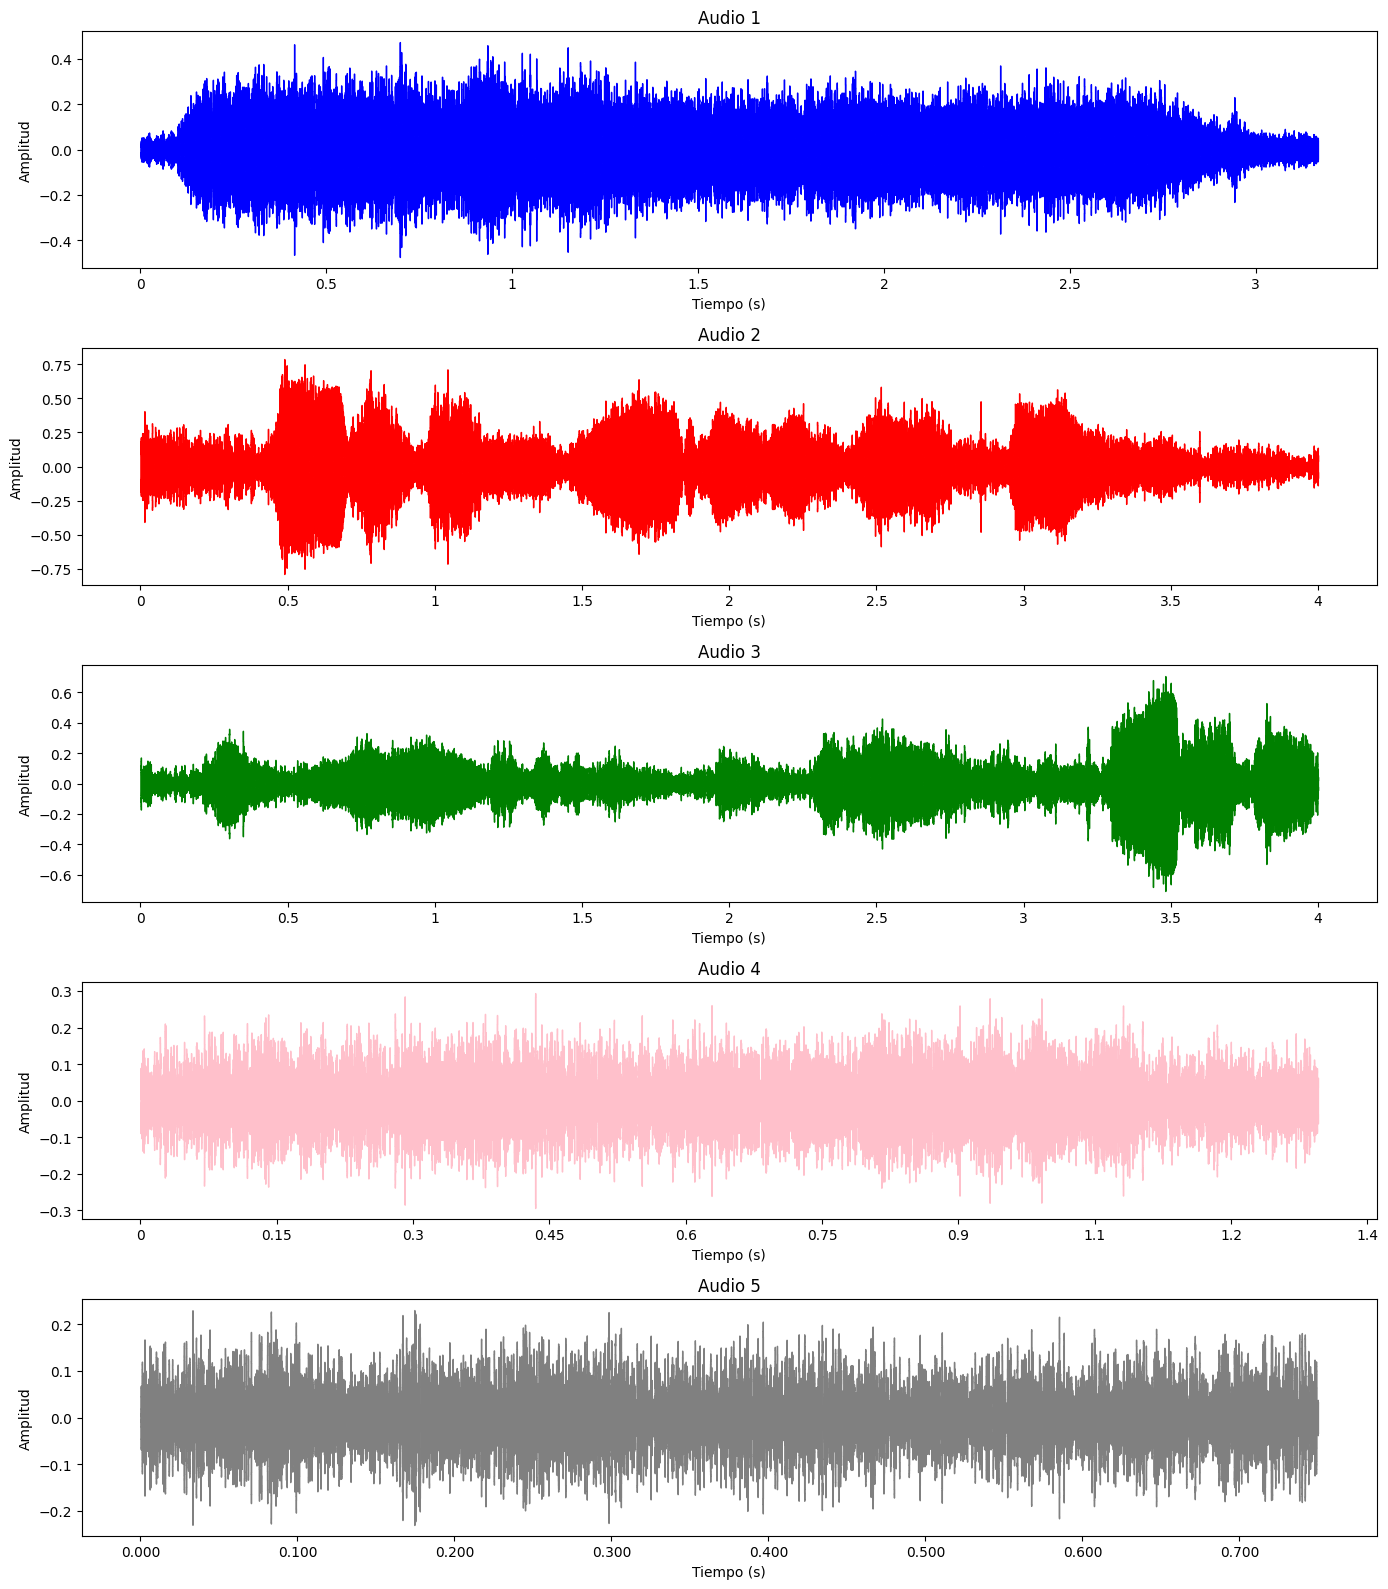
\includegraphics[width=15cm]{Images/Amplitudes}
	\caption{grafico de frecuencias y distribución}
	\label{fig:FyD}
\end{figure}

\begin{figure}[!h]
	\centering
	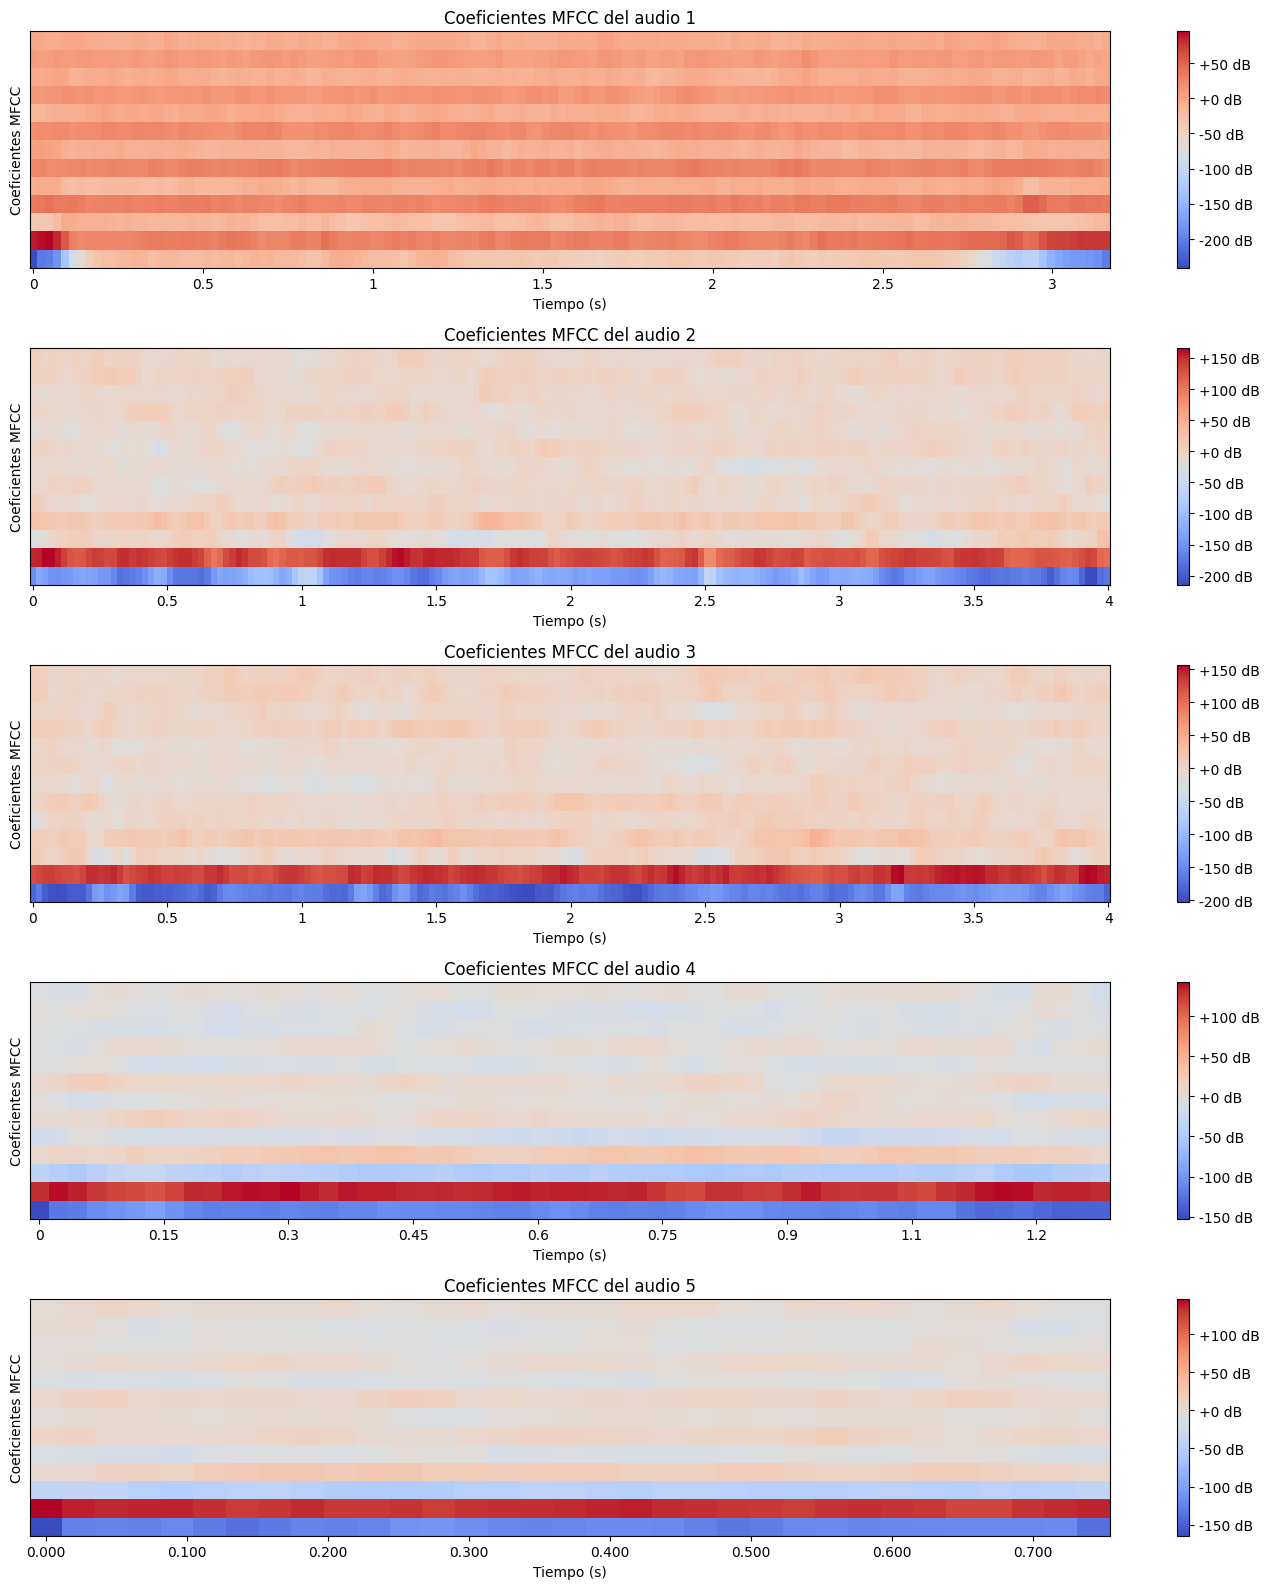
\includegraphics[width=15cm]{Images/Coeficientes}
	\caption{grafico de frecuencias y distribución}
	\label{fig:FyD}
\end{figure}

\begin{figure}[!h]
	\centering
	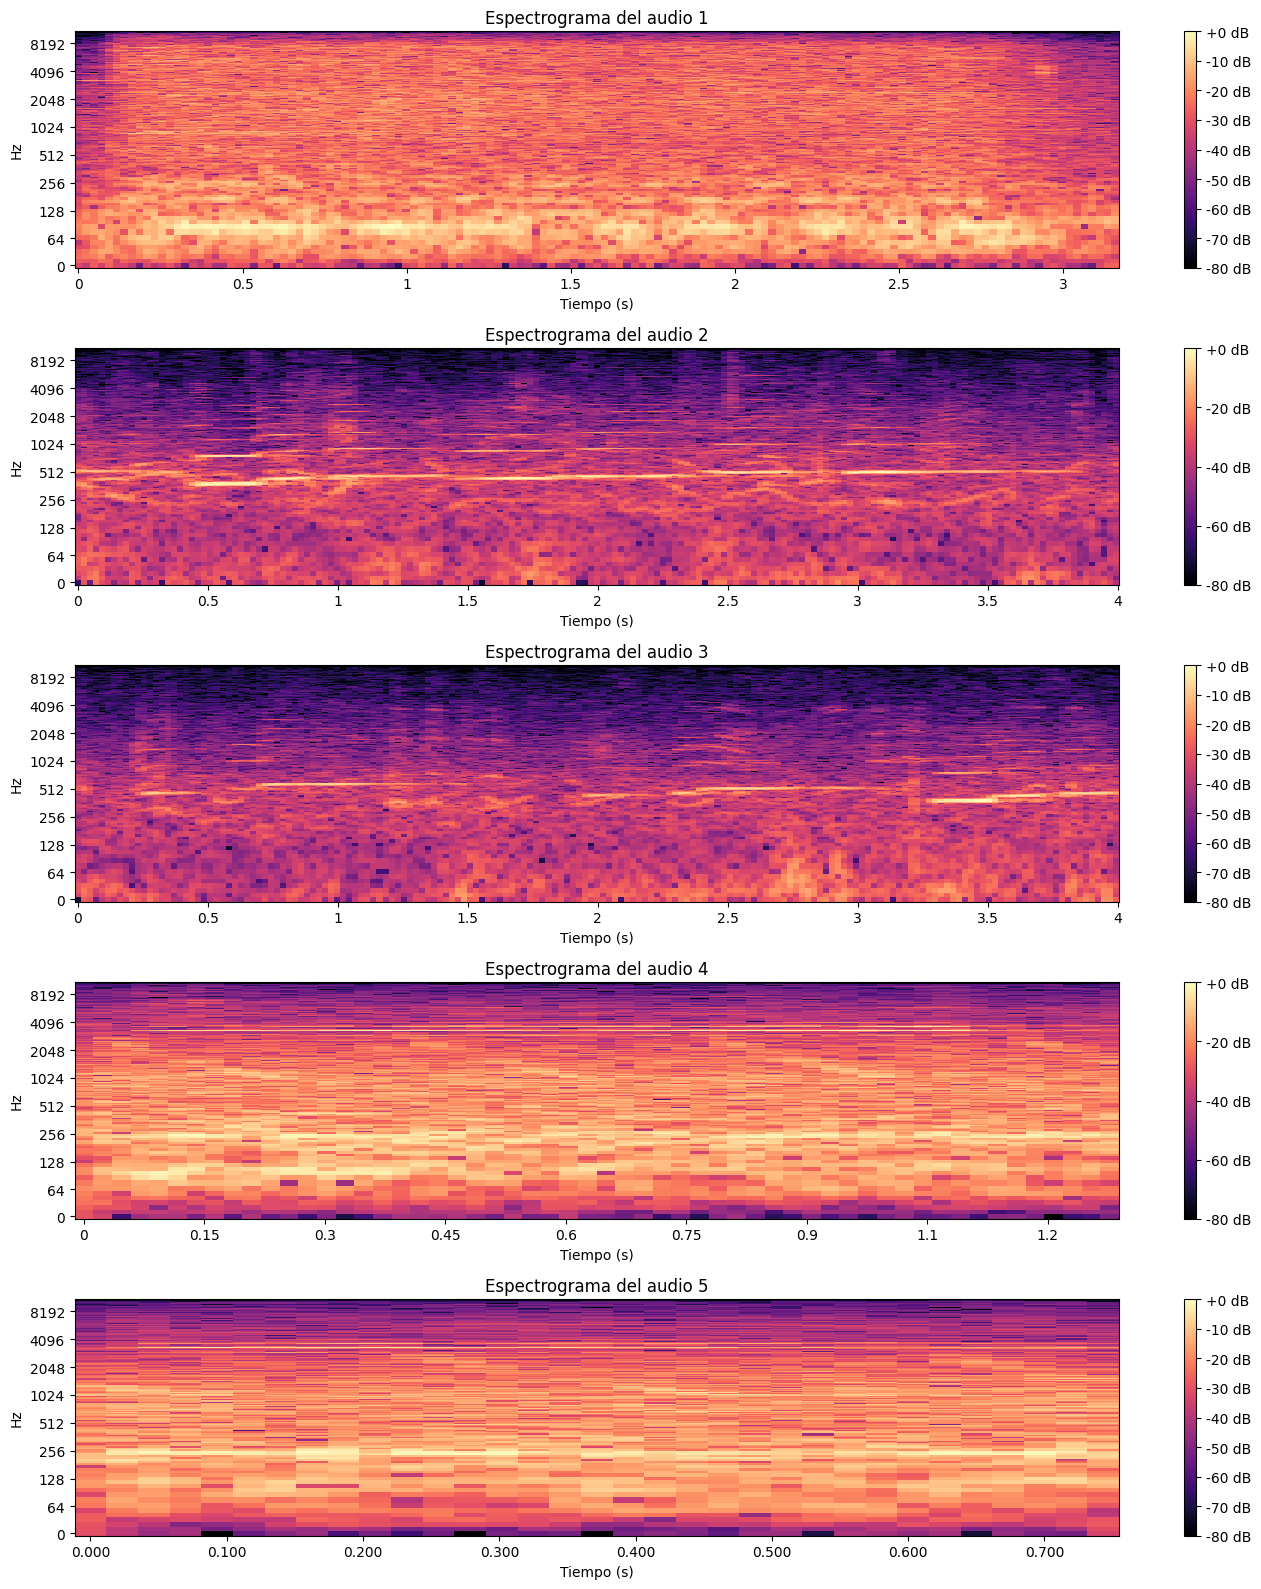
\includegraphics[width=15cm]{Images/Espectrograma}
	\caption{grafico de frecuencias y distribución}
	\label{fig:FyD}
\end{figure}

\begin{figure}[!h]
	\centering
	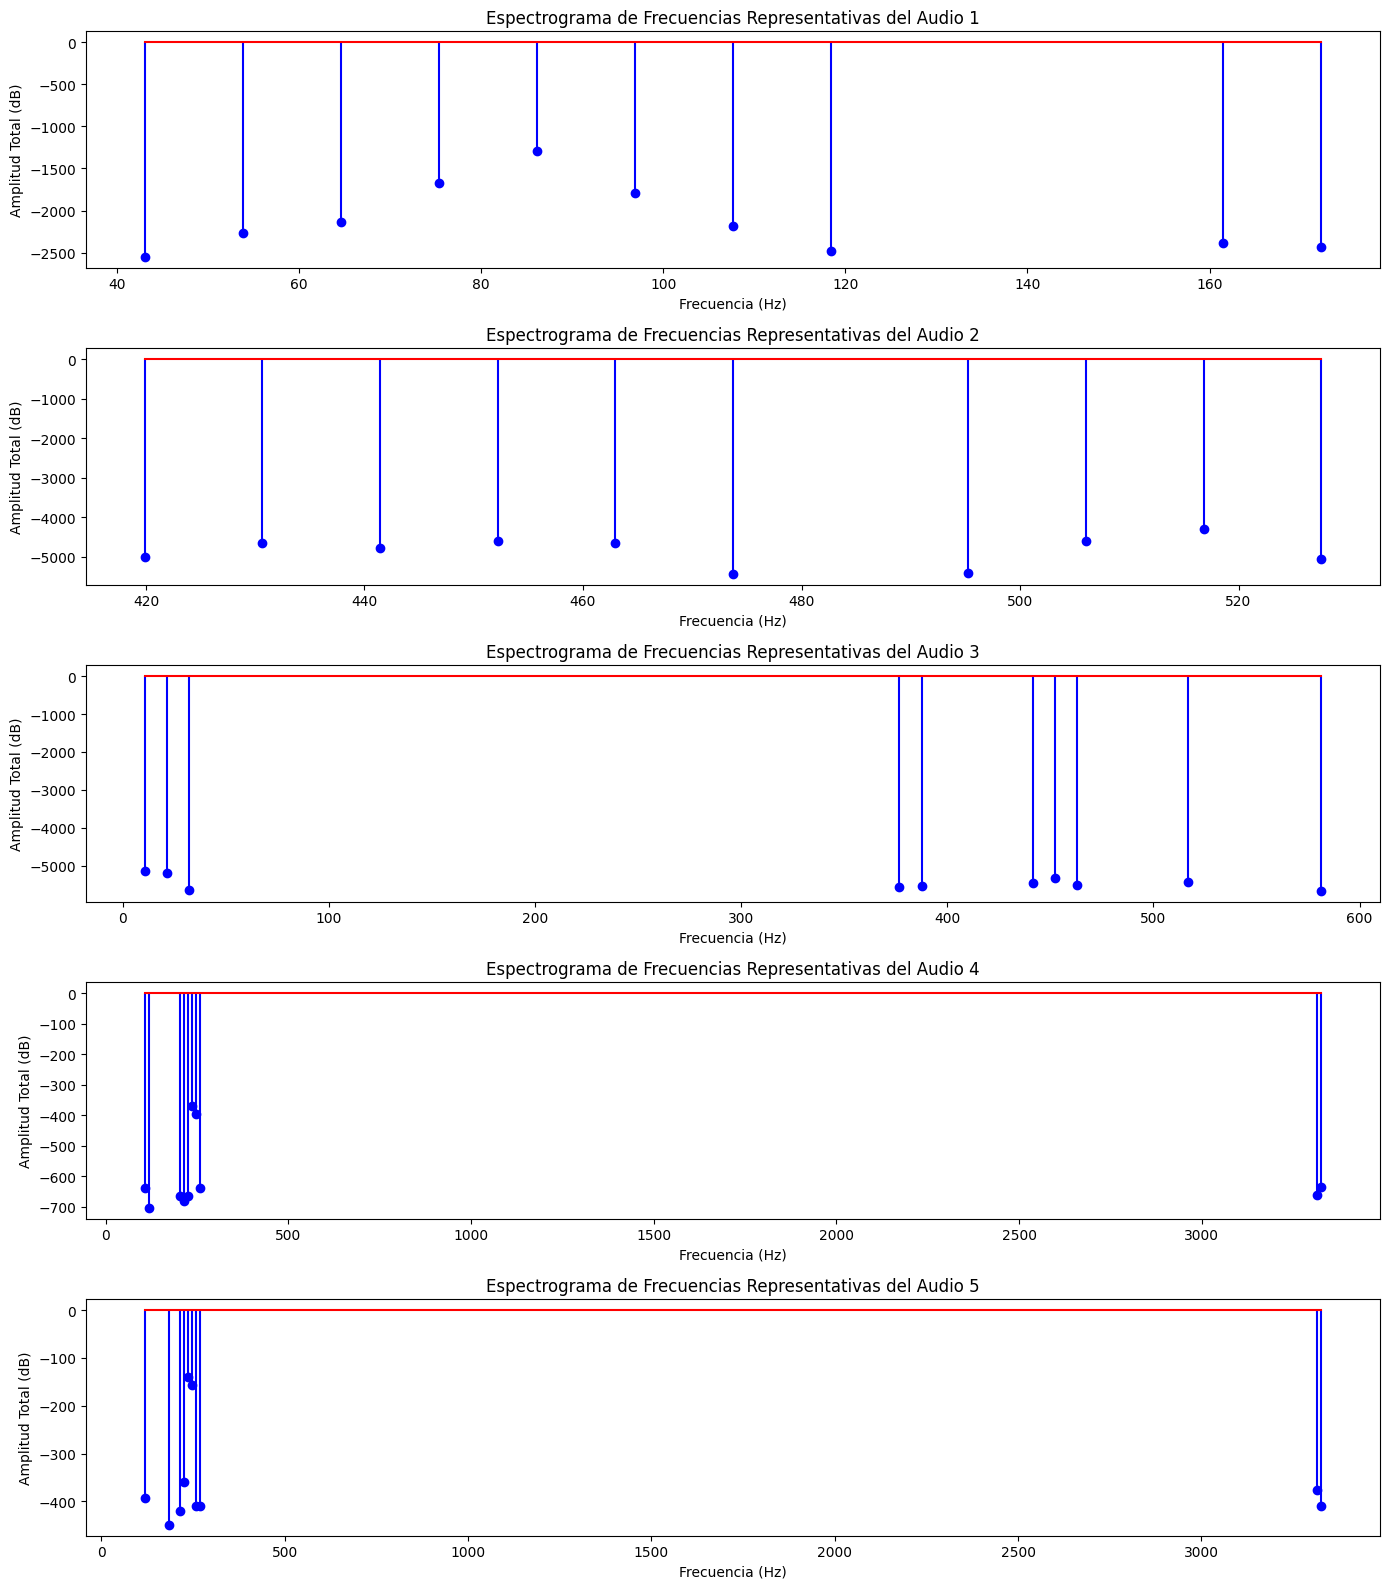
\includegraphics[width=15cm]{Images/Frecuencias_representativas}
	\caption{grafico de frecuencias y distribución}
	\label{fig:FyD}
\end{figure}



\chapter{Conclusiones}

